% ============================================================================
% Caffeine Engine — Internal Technical Reference
%
% Purpose: Formal academic-style document covering the mathematical,
%          theoretical, and architectural foundations of every core system
%          in the Caffeine Engine. Intended for contributors who wish to
%          understand the engine at a deep level, and as a specification
%          reference that governs all future core implementations.
%
% Language: English
% Compiler: pdfLaTeX or LuaLaTeX
%
% Structure:
%   main.tex          — preamble, page setup, document root
%   front/cover.tex   — title page
%   front/abstract.tex — abstract + ToC
%   chapters/NN-*.tex — one file per chapter
% ============================================================================

\documentclass[12pt, a4paper]{report}

% ── Geometry ─────────────────────────────────────────────────────────────────
\usepackage[left=3cm, right=2cm, top=3cm, bottom=2cm]{geometry}

% ── Typography ────────────────────────────────────────────────────────────────
\usepackage[T1]{fontenc}
\usepackage[utf8]{inputenc}
\usepackage{helvet}
\renewcommand{\familydefault}{\sfdefault}
\usepackage{setspace}
\onehalfspacing
\usepackage{microtype}

% ── Colour ────────────────────────────────────────────────────────────────────
\usepackage{xcolor}
\definecolor{darkblue}{RGB}{0,32,96}
\definecolor{codebg}{RGB}{245,245,248}
\definecolor{rulegray}{RGB}{180,180,195}
\definecolor{accentblue}{RGB}{60,100,200}

% ── Section styling ───────────────────────────────────────────────────────────
\usepackage{titlesec}
\titleformat{\chapter}[display]
  {\color{darkblue}\sffamily\huge\bfseries}
  {\color{darkblue}\chaptertitlename\ \thechapter}{12pt}{}
\titleformat{\section}
  {\color{darkblue}\sffamily\Large\bfseries}{\thesection}{1em}{}
\titleformat{\subsection}
  {\color{darkblue}\sffamily\large\bfseries}{\thesubsection}{1em}{}
\titleformat{\subsubsection}
  {\sffamily\normalsize\bfseries}{\thesubsubsection}{1em}{}

% ── Mathematics ───────────────────────────────────────────────────────────────
\usepackage{amsmath, amssymb, amsthm}
\usepackage{mathtools}
\theoremstyle{definition}
\newtheorem{definition}{Definition}[section]
\theoremstyle{remark}
\newtheorem{remark}{Remark}[section]
\newtheorem{invariant}{Invariant}[section]

% ── Code listings ─────────────────────────────────────────────────────────────
\usepackage{listings}
\lstset{
  basicstyle=\ttfamily\small,
  backgroundcolor=\color{codebg},
  frame=single,
  framerule=0.4pt,
  rulecolor=\color{rulegray},
  breaklines=true,
  breakatwhitespace=true,
  showstringspaces=false,
  tabsize=4,
  captionpos=b,
  numbers=left,
  numberstyle=\tiny\color{gray},
  numbersep=6pt,
  keywordstyle=\color{accentblue}\bfseries,
  commentstyle=\color{gray}\itshape,
  stringstyle=\color{darkblue},
  language=C++
}

% ── Hyperlinks & PDF metadata ─────────────────────────────────────────────────
\usepackage[hidelinks, bookmarks=true]{hyperref}
\hypersetup{
  pdftitle={Caffeine Engine -- Internal Technical Reference},
  pdfauthor={Caffeine Engine Contributors},
  pdfsubject={Game Engine Architecture, Mathematics, Systems Programming}
}

% ── Tables & figures ──────────────────────────────────────────────────────────
\usepackage{booktabs}
\usepackage{longtable}
\usepackage{array}
\usepackage{multirow}
\usepackage{graphicx}
\usepackage{float}
\usepackage{caption}
\captionsetup{font=small, labelfont=bf}

% ── Header / footer ───────────────────────────────────────────────────────────
\usepackage{fancyhdr}
\pagestyle{fancy}
\fancyhf{}
\fancyhead[L]{\small\color{rulegray}\leftmark}
\fancyhead[R]{\small\color{rulegray}Caffeine Engine — Internal Reference}
\fancyfoot[R]{\thepage}
\renewcommand{\headrulewidth}{0.4pt}
\renewcommand{\headrule}{\color{rulegray}\hrule width\headwidth height\headrulewidth}

% ── Page numbering ────────────────────────────────────────────────────────────
\usepackage{etoolbox}

% ── Utility ───────────────────────────────────────────────────────────────────
\usepackage{enumitem}
\usepackage{tcolorbox}
\tcbuselibrary{breakable}
\usepackage{tikz}

% ── Custom environments ───────────────────────────────────────────────────────
\newtcolorbox{specbox}[1]{
  colback=codebg, colframe=darkblue!40,
  fonttitle=\sffamily\bfseries,
  title=#1, breakable
}

% =============================================================================
\begin{document}

% ── Pre-textual pages (Roman numerals) ───────────────────────────────────────
\pagenumbering{roman}
\pagestyle{empty}

% ============================================================================
% COVER PAGE
% ============================================================================
\begin{titlepage}
  \centering
  \vspace*{2cm}

  {\color{darkblue}\sffamily\Huge\bfseries CAFFEINE ENGINE}\\[0.6em]
  {\color{darkblue}\sffamily\Large\bfseries INTERNAL TECHNICAL REFERENCE}\\[1.2em]
  {\sffamily\large Core Systems, Mathematics, and Architectural Foundations}

  \vspace{2.5cm}

  {\sffamily\normalsize
    A formal specification covering the mathematical basis and implementation
    rationale of every subsystem in the Caffeine Engine.
    This document is the authoritative reference for contributors and serves as
    the planning specification for all future core and UI implementations.
  }

  \vfill

  \begin{tabular}{ll}
    \textbf{Repository} & \texttt{devscafecommunity/caffeine} \\[0.4em]
    \textbf{Standard}   & C++20, SDL3, ImGui \\[0.4em]
    \textbf{Platform}   & Windows / Linux / macOS (x64) \\[0.4em]
    \textbf{Revision}   & 2026 \\
  \end{tabular}

  \vspace{1.5cm}
  {\small\color{gray} This document is internal. It does not duplicate the public
  README or user guide; its sole purpose is deep technical understanding.}
\end{titlepage}

% ============================================================================
% ABSTRACT + TABLE OF CONTENTS
% ============================================================================
\chapter*{Abstract}
\addcontentsline{toc}{chapter}{Abstract}

The Caffeine Engine is a custom C++20 game engine built over SDL3, designed
with explicit control over hardware, memory, and concurrency as primary
objectives. This document provides the complete internal specification of its
core systems: the primitive type layer, mathematical library
(vectors, matrices, quaternions), custom memory allocators, generic
container implementations, the Entity-Component-System (ECS) architecture,
a work-stealing job system, a 2D rigid-body physics engine, a spatial audio
system, a binary asset pipeline, and the software-rasterised 3D/Isometric
scene viewport with its projection mathematics and transform gizmo framework.

Each system is described at the level required to understand its design
decisions, prove its correctness, and extend it safely. Formulas are
presented in their complete mathematical form; implementation details follow
directly from the theory. This document is both a teaching resource and a
binding specification: any proposed change to a described system must be
reconciled with the invariants stated here before implementation begins.

\bigskip
\textbf{Keywords:} game engine, ECS, memory allocators, quaternions,
work-stealing scheduler, impulse-based physics, software projection,
asset pipeline, C++20.

% ── Table of contents / figures / tables ─────────────────────────────────────
\pagestyle{plain}
\tableofcontents
\listoffigures
\listoftables


% ── Body (Arabic numerals) ────────────────────────────────────────────────────
\cleardoublepage
\pagenumbering{arabic}
\setcounter{page}{1}
\pagestyle{fancy}

% ============================================================================
\chapter{Introduction}
% ============================================================================

\section{Philosophy}

Caffeine Engine is built under a single principle: \emph{transparency}.
Every byte that passes through the CPU must be accountable to the
programmer. This philosophy manifests in three concrete decisions.

\begin{itemize}[leftmargin=1.5em]
  \item \textbf{Zero-dependency standard library.} The engine replaces
        \texttt{std} containers with its own implementations tuned for
        game-loop access patterns (cache-friendly sequential iteration,
        allocator-aware growth, no hidden heap traffic).

  \item \textbf{Data-oriented design.} Entities are not objects; they are
        integer identifiers. Components are plain-old-data structs stored in
        contiguous typed pools. This layout maximises SIMD and cache line
        utilisation during system updates.

  \item \textbf{Explicit concurrency.} No implicit background threads.
        The job system is the single scheduling primitive; callers declare
        dependencies explicitly through barriers and handles.
\end{itemize}

\section{Document Structure}

Each subsequent chapter covers one major subsystem. The ordering follows
the dependency graph: fundamental types and mathematics are presented first,
followed by memory, containers, ECS, threading, domain systems (physics,
audio), the asset pipeline, and finally the editor viewport. Each chapter
concludes with a table of invariants that any future implementation must
preserve.

\section{Notation Conventions}

Throughout this document, the following notation is used consistently.

\begin{itemize}[leftmargin=1.5em]
  \item Scalars: italic Latin letters --- $a, b, t, \theta$.
  \item Vectors: bold lower-case --- $\mathbf{v}, \mathbf{u}, \mathbf{n}$.
  \item Matrices: bold upper-case --- $\mathbf{M}, \mathbf{R}$.
  \item Quaternions: calligraphic --- $\mathcal{q}$.
  \item Unit vectors: hat notation --- $\hat{\mathbf{v}}$.
  \item Column-major storage is assumed unless stated otherwise.
  \item Code identifiers appear in \texttt{monospace}.
\end{itemize}

% ============================================================================
\chapter{Type System and Platform Abstractions}
% ============================================================================

\section{Primitive Types (\texttt{Types.hpp})}

All numeric types in the engine are defined as explicit-width aliases in
\texttt{src/core/Types.hpp}. The rationale is binary portability: the C++
standard permits \texttt{int} to be 16- or 32-bit depending on the platform;
the engine must never depend on implicit widths.

\begin{table}[H]
\centering
\caption{Caffeine primitive type aliases}
\begin{tabular}{lll}
\toprule
\textbf{Alias} & \textbf{Underlying type} & \textbf{Width} \\
\midrule
\texttt{i8 / u8}   & \texttt{int8\_t / uint8\_t}   & 8 bit  \\
\texttt{i16 / u16} & \texttt{int16\_t / uint16\_t} & 16 bit \\
\texttt{i32 / u32} & \texttt{int32\_t / uint32\_t} & 32 bit \\
\texttt{i64 / u64} & \texttt{int64\_t / uint64\_t} & 64 bit \\
\texttt{f32}       & \texttt{float}                & 32 bit IEEE 754 \\
\texttt{f64}       & \texttt{double}               & 64 bit IEEE 754 \\
\texttt{usize}     & \texttt{std::size\_t}         & Platform pointer-width \\
\texttt{isize}     & \texttt{std::ptrdiff\_t}      & Platform pointer-width \\
\bottomrule
\end{tabular}
\end{table}

Every width is validated by \texttt{static\_assert} at compile time.
The consequence is that \emph{inclusion of \texttt{Types.hpp} is the first
gate for all cross-platform build failures}: if the platform violates any
width, the translation unit refuses to compile.

\section{Compiler Abstraction (\texttt{Compiler.hpp})}

Platform-specific compiler directives are isolated in a single header so
that all engine source files are compiler-agnostic. The macros provided
include \texttt{CF\_INLINE} (\texttt{\_\_forceinline} on MSVC;
\texttt{\_\_attribute\_\_((always\_inline))} on GCC/Clang),
\texttt{CF\_NORETURN}, \texttt{CF\_LIKELY / CF\_UNLIKELY} (branch hints),
and \texttt{CF\_BUILTIN\_TRAP} (hard abort in debug builds).

\section{Assertions}

The macro \texttt{CF\_ASSERT(cond, msg)} is active in debug builds
(\texttt{CF\_DEBUG} defined) and compiles to a no-op in release builds.
When an assertion fires it calls \texttt{Caffeine::assertFailed}, which
invokes \texttt{CF\_BUILTIN\_TRAP()} causing an immediate hardware trap.
This is deliberately brutal: masked failures in debug are more dangerous
than hard crashes.

\begin{specbox}{Invariant 2.1 --- Assert semantics}
  No assertion shall be removed to silence a false positive.
  If \texttt{CF\_ASSERT} fires, the precondition it guards must be fixed at
  the call site, not at the assertion.
\end{specbox}

\section{Timing (\texttt{Timer.hpp})}

The \texttt{Timer} class wraps \texttt{std::chrono::high\_resolution\_clock}
and exposes nanosecond-precision \texttt{TimePoint} values. The
\texttt{Duration} struct carries time as a 64-bit \texttt{double} in seconds,
with helper conversions to milliseconds, microseconds, and nanoseconds.

The \texttt{ScopeTimer} RAII guard is used for fine-grained profiling of
editor sub-systems. Its destructor stops the timer and records the elapsed
duration; the name string is a static pointer (not heap-allocated) to keep
the measurement overhead negligible.

% ============================================================================
\chapter{Mathematics Library}
% ============================================================================

\section{Overview}

The mathematics library in \texttt{src/math/} provides the complete set of
primitive geometric types used throughout the engine. All types are plain
structs with no virtual methods, no heap allocation, and scalar fields
only --- compatible with \texttt{memcpy} serialisation and SIMD reinterpretation
on compilers that respect standard-layout guarantees.

\section{Two-Dimensional Vectors (\texttt{Vec2})}

\begin{definition}[2-Vector]
A two-dimensional vector $\mathbf{v} \in \mathbb{R}^2$ is defined as
$\mathbf{v} = (x, y)$ where $x, y \in \mathbb{R}$.
\end{definition}

The \texttt{Vec2} struct stores two \texttt{f32} components. The fundamental
operations and their implementations are:

\begin{align}
  \text{Dot product:} \quad & \mathbf{u} \cdot \mathbf{v} = u_x v_x + u_y v_y \\
  \text{Squared length:} \quad & |\mathbf{v}|^2 = \mathbf{v} \cdot \mathbf{v} \\
  \text{Euclidean length:} \quad & |\mathbf{v}| = \sqrt{|\mathbf{v}|^2} \\
  \text{Normalisation:} \quad & \hat{\mathbf{v}} =
    \begin{cases} \mathbf{v} / |\mathbf{v}| & \text{if } |\mathbf{v}| > 0 \\ \mathbf{0} & \text{otherwise} \end{cases}
\end{align}

The implementation guards against division by zero in both
\texttt{length()} and \texttt{normalized()} by checking
$|\mathbf{v}|^2 > 0$ before taking the square root or dividing.

\section{Three-Dimensional Vectors (\texttt{Vec3})}

\begin{definition}[3-Vector]
A three-dimensional vector $\mathbf{v} \in \mathbb{R}^3$ is
$\mathbf{v} = (x, y, z)$ with components $x, y, z \in \mathbb{R}$.
\end{definition}

In addition to the operations shared with \texttt{Vec2}, \texttt{Vec3}
provides:

\begin{align}
  \text{Cross product:} \quad
  \mathbf{u} \times \mathbf{v} &=
  \begin{pmatrix} u_y v_z - u_z v_y \\ u_z v_x - u_x v_z \\ u_x v_y - u_y v_x \end{pmatrix}
\end{align}

The cross product is anticommutative: $\mathbf{u} \times \mathbf{v} = -(\mathbf{v} \times \mathbf{u})$.
It is used extensively in matrix construction (\texttt{lookAt}),
Gram-Schmidt orthonormalisation, and quaternion rotation.

Static convenience accessors \texttt{Vec3::forward()}, \texttt{Vec3::up()},
and \texttt{Vec3::right()} return the canonical basis vectors
$(0,0,1)$, $(0,1,0)$, and $(1,0,0)$ respectively.

\section{Four-Dimensional Vectors (\texttt{Vec4})}

\texttt{Vec4} extends \texttt{Vec3} with a homogeneous $w$ coordinate.
It is used as the input to 4$\times$4 matrix multiplications (points have
$w = 1$; directions have $w = 0$) and as a colour representation
$(r, g, b, a)$.

\section{4$\times$4 Matrices (\texttt{Mat4})}

\subsection{Storage Layout}

\texttt{Mat4} stores 16 \texttt{f32} values in a flat array \texttt{m[16]}
using \emph{column-major} order. Element $(row, col)$ maps to
$\texttt{m}[col \cdot 4 + row]$. This layout is compatible with the
OpenGL / Vulkan column-major convention and allows a matrix column to
be loaded as a single 128-bit SIMD register.

\subsection{Fundamental Transforms}

\subsubsection{Translation}

\[
\mathbf{T}(t_x, t_y, t_z) =
\begin{pmatrix}
1 & 0 & 0 & t_x \\
0 & 1 & 0 & t_y \\
0 & 0 & 1 & t_z \\
0 & 0 & 0 & 1
\end{pmatrix}
\]

\subsubsection{Scale}

\[
\mathbf{S}(s_x, s_y, s_z) =
\begin{pmatrix}
s_x & 0   & 0   & 0 \\
0   & s_y & 0   & 0 \\
0   & 0   & s_z & 0 \\
0   & 0   & 0   & 1
\end{pmatrix}
\]

\subsubsection{Rotation about Z, Y, X}

\[
\mathbf{R}_z(\theta) =
\begin{pmatrix}
\cos\theta & -\sin\theta & 0 & 0 \\
\sin\theta &  \cos\theta & 0 & 0 \\
0          & 0           & 1 & 0 \\
0          & 0           & 0 & 1
\end{pmatrix}
\quad
\mathbf{R}_y(\theta) =
\begin{pmatrix}
 \cos\theta & 0 & \sin\theta & 0 \\
 0          & 1 & 0          & 0 \\
-\sin\theta & 0 & \cos\theta & 0 \\
 0          & 0 & 0          & 1
\end{pmatrix}
\]

\[
\mathbf{R}_x(\theta) =
\begin{pmatrix}
1 & 0          & 0           & 0 \\
0 & \cos\theta & -\sin\theta & 0 \\
0 & \sin\theta &  \cos\theta & 0 \\
0 & 0          & 0           & 1
\end{pmatrix}
\]

\subsubsection{Orthographic Projection}

\[
\mathbf{P}_\text{ortho} =
\begin{pmatrix}
\dfrac{2}{r-l} & 0 & 0 & -\dfrac{r+l}{r-l} \\[6pt]
0 & \dfrac{2}{t-b} & 0 & -\dfrac{t+b}{t-b} \\[6pt]
0 & 0 & -\dfrac{2}{f-n} & -\dfrac{f+n}{f-n} \\[6pt]
0 & 0 & 0 & 1
\end{pmatrix}
\]

where $l, r, b, t, n, f$ are the left, right, bottom, top, near, and far
clipping planes.

\subsubsection{Perspective Projection}

Let $\theta_y$ be the vertical field-of-view angle and $a$ the
aspect ratio $w/h$.

\[
\mathbf{P}_\text{persp} =
\begin{pmatrix}
\dfrac{1}{a \tan(\theta_y/2)} & 0 & 0 & 0 \\[8pt]
0 & \dfrac{1}{\tan(\theta_y/2)} & 0 & 0 \\[8pt]
0 & 0 & -\dfrac{f+n}{f-n} & -1 \\[4pt]
0 & 0 & -\dfrac{2fn}{f-n} & 0
\end{pmatrix}
\]

\subsubsection{Look-At View Matrix}

Given eye position $\mathbf{e}$, target $\mathbf{t}$, and world up
$\mathbf{u}_w$:

\begin{align}
\mathbf{f} &= \widehat{\mathbf{t} - \mathbf{e}} \quad (\text{forward}) \\
\mathbf{r} &= \widehat{\mathbf{f} \times \mathbf{u}_w} \quad (\text{right}) \\
\mathbf{u} &= \mathbf{r} \times \mathbf{f} \quad (\text{corrected up}) \\
\mathbf{V} &=
\begin{pmatrix}
r_x & r_y & r_z & -\mathbf{r}\cdot\mathbf{e} \\
u_x & u_y & u_z & -\mathbf{u}\cdot\mathbf{e} \\
-f_x & -f_y & -f_z & \mathbf{f}\cdot\mathbf{e} \\
0 & 0 & 0 & 1
\end{pmatrix}
\end{align}

\subsection{Matrix Inversion}

\texttt{Mat4::inverted()} implements the \textbf{cofactor expansion} method
(Cram\'er's rule). The adjugate matrix $\text{adj}(\mathbf{M})$ is computed
element-by-element as the transpose of the cofactor matrix. The inverse is:

\[
\mathbf{M}^{-1} = \frac{1}{\det(\mathbf{M})} \cdot \text{adj}(\mathbf{M})
\]

If $|\det(\mathbf{M})| < 10^{-6}$, the matrix is considered singular and
the identity matrix is returned. This avoids undefined behaviour at the
cost of silently returning an incorrect inverse; callers that construct
degenerate matrices bear responsibility for that degeneracy.

\section{Quaternions (\texttt{Quat})}

\subsection{Mathematical Foundation}

\begin{definition}[Quaternion]
A quaternion $\mathcal{q} \in \mathbb{H}$ is an element of the form
$\mathcal{q} = w + xi + yj + zk$ where $w, x, y, z \in \mathbb{R}$ and
the imaginary units satisfy $i^2 = j^2 = k^2 = ijk = -1$ (Hamilton convention).
\end{definition}

The engine stores quaternions as $(x, y, z, w)$ in memory, where $w$ is
the scalar (real) part and $(x, y, z)$ is the vector (imaginary) part
$\mathcal{q}_v$.

A \textbf{unit quaternion} ($|\mathcal{q}| = 1$) represents a rotation.
The rotation by angle $\theta$ around unit axis $\hat{\mathbf{n}}$ is:

\begin{equation}
\mathcal{q} = \left(\hat{\mathbf{n}} \sin\tfrac{\theta}{2},\ \cos\tfrac{\theta}{2}\right)
\label{eq:quat-axis-angle}
\end{equation}

\subsection{Quaternion Product (Hamilton Product)}

\begin{align}
\mathcal{q}_1 \cdot \mathcal{q}_2 &=
(w_1 w_2 - \mathcal{q}_{v1} \cdot \mathcal{q}_{v2},\
 w_1 \mathcal{q}_{v2} + w_2 \mathcal{q}_{v1} + \mathcal{q}_{v1} \times \mathcal{q}_{v2})
\end{align}

In component form (the implementation in \texttt{operator*}):
\begin{align}
x' &= w_1 x_2 + x_1 w_2 + y_1 z_2 - z_1 y_2 \\
y' &= w_1 y_2 - x_1 z_2 + y_1 w_2 + z_1 x_2 \\
z' &= w_1 z_2 + x_1 y_2 - y_1 x_2 + z_1 w_2 \\
w' &= w_1 w_2 - x_1 x_2 - y_1 y_2 - z_1 z_2
\end{align}

The product $\mathcal{q}_1 \cdot \mathcal{q}_2$ applies $\mathcal{q}_2$ first,
then $\mathcal{q}_1$ --- the same composition order as matrix multiplication.

\subsection{Vector Rotation}

Rotating vector $\mathbf{v}$ by unit quaternion $\mathcal{q}$ is equivalent to
$\mathcal{q} \cdot (0, \mathbf{v}) \cdot \mathcal{q}^{-1}$.
The efficient formulation avoids the full product by exploiting the identity:

\begin{equation}
\mathbf{v}' = \mathbf{v} + 2\,\mathcal{q}_v \times (\mathcal{q}_v \times \mathbf{v} + w\,\mathbf{v})
\label{eq:quat-rotate}
\end{equation}

This requires only two cross products instead of two full quaternion products,
reducing the operation from 28 multiplications to 15.

\subsection{Quaternion to Rotation Matrix}

For a unit quaternion $\mathcal{q} = (x, y, z, w)$:

\[
\mathbf{R} =
\begin{pmatrix}
1 - 2(y^2+z^2) & 2(xy - zw)     & 2(xz + yw) \\
2(xy + zw)     & 1 - 2(x^2+z^2) & 2(yz - xw) \\
2(xz - yw)     & 2(yz + xw)     & 1 - 2(x^2+y^2)
\end{pmatrix}
\]

This matrix satisfies $\mathbf{R}\mathbf{v} = \mathcal{q} \cdot \mathbf{v} \cdot \mathcal{q}^{-1}$
for any vector $\mathbf{v}$ and $\mathbf{R}\mathbf{R}^T = \mathbf{I}$
for unit quaternions.

\subsection{Rotation Matrix to Quaternion (Shoemake 1987)}

The trace-based algorithm of Ken Shoemake selects the numerically largest
diagonal element to avoid division by near-zero values.
Let $\text{tr} = R_{00} + R_{11} + R_{22}$.

\textbf{Case} $\text{tr} > 0$:
\[
s = 2\sqrt{\text{tr}+1}, \quad
w = s/4, \quad
x = (R_{21}-R_{12})/s, \quad
y = (R_{02}-R_{20})/s, \quad
z = (R_{10}-R_{01})/s
\]

\textbf{Case} $R_{00}$ is the largest diagonal:
\[
s = 2\sqrt{1+R_{00}-R_{11}-R_{22}}, \quad
x = s/4, \quad
y = (R_{01}+R_{10})/s, \quad
z = (R_{02}+R_{20})/s, \quad
w = (R_{21}-R_{12})/s
\]

Analogous formulae apply when $R_{11}$ or $R_{22}$ are largest.

\subsection{Euler Angles (ZYX Tait-Bryan Convention)}

The engine uses the ZYX (intrinsic) convention: roll (Z) applied first,
then pitch (X), then yaw (Y) last.
Given angles $\phi$ (roll), $\theta$ (pitch), $\psi$ (yaw):

\begin{align}
  w &= \cos(\phi/2)\cos(\psi/2)\cos(\theta/2) + \sin(\phi/2)\sin(\psi/2)\sin(\theta/2) \\
  x &= \cos(\phi/2)\cos(\psi/2)\sin(\theta/2) - \sin(\phi/2)\sin(\psi/2)\cos(\theta/2) \\
  y &= \cos(\phi/2)\sin(\psi/2)\cos(\theta/2) + \sin(\phi/2)\cos(\psi/2)\sin(\theta/2) \\
  z &= \sin(\phi/2)\cos(\psi/2)\cos(\theta/2) - \cos(\phi/2)\sin(\psi/2)\sin(\theta/2)
\end{align}

The inverse (quaternion to Euler) extracts angles from the rotation matrix
rows via \texttt{atan2} and \texttt{asin}:

\begin{align}
  \psi  &= \arcsin\!\bigl(-2(xz - wy)\bigr) \quad (\text{yaw}) \\
  \theta &= \operatorname{atan2}\!\bigl(2(yz+wx),\, 1-2(x^2+y^2)\bigr) \quad (\text{pitch}) \\
  \phi  &= \operatorname{atan2}\!\bigl(2(xy+wz),\, 1-2(y^2+z^2)\bigr) \quad (\text{roll})
\end{align}

Gimbal lock occurs at $\psi = \pm\pi/2$ and is not resolved in the current
implementation; users should prefer quaternions for continuous rotation.

\subsection{Spherical Linear Interpolation (SLERP)}

\begin{equation}
\text{SLERP}(\mathcal{q}_a, \mathcal{q}_b, t)
= \frac{\sin((1-t)\Omega)}{\sin\Omega}\,\mathcal{q}_a
+ \frac{\sin(t\Omega)}{\sin\Omega}\,\mathcal{q}_b
\label{eq:slerp}
\end{equation}

where $\Omega = \arccos(|\mathcal{q}_a \cdot \mathcal{q}_b|)$.
The shortest arc is guaranteed by negating $\mathcal{q}_b$ when
$\mathcal{q}_a \cdot \mathcal{q}_b < 0$.
When $\mathcal{q}_a \cdot \mathcal{q}_b > 0.9999$, linear interpolation
(NLERP) is used to avoid the numerical instability of $\sin\Omega \approx 0$.

\subsection{Normalised Linear Interpolation (NLERP)}

\begin{equation}
\text{NLERP}(\mathcal{q}_a, \mathcal{q}_b, t)
= \frac{(1-t)\,\mathcal{q}_a + t\,\mathcal{q}_b}{|(1-t)\,\mathcal{q}_a + t\,\mathcal{q}_b|}
\label{eq:nlerp}
\end{equation}

NLERP does not maintain constant angular velocity --- interpolation speed
is faster near the midpoint --- but is significantly cheaper (one
normalisation vs.\ two \texttt{sinf}/\texttt{atan2f} evaluations).

\section{Mathematical Utilities (\texttt{Math.hpp})}

The \texttt{Caffeine::Math} namespace provides scalar utility functions.
Key values:

\begin{align*}
  \pi &= 3.14159265358979323846 \\
  \tau &= 2\pi \\
  e &= 2.71828182845904523536
\end{align*}

\subsubsection{Smoothstep}

The cubic Hermite interpolant used for smooth transitions:

\begin{equation}
\text{smoothstep}(e_0, e_1, x)
= t^2(3 - 2t), \quad t = \text{saturate}\!\left(\frac{x - e_0}{e_1 - e_0}\right)
\end{equation}

\subsubsection{Next Power of Two}

\begin{lstlisting}[caption={Bit-manipulation power-of-two rounding}]
usize nextPowerOfTwo(usize v) {
    --v;
    v |= v >> 1;  v |= v >> 2;
    v |= v >> 4;  v |= v >> 8;
    v |= v >> 16;
    return v + 1;
}
\end{lstlisting}

This bit-spreading algorithm fills all lower bits of $v-1$ with 1s,
then adds 1. It runs in $O(\log_2 w)$ operations where $w$ is the word width.

% ============================================================================
\chapter{Memory Management}
% ============================================================================

\section{The Allocator Interface (\texttt{IAllocator})}

All allocators implement the pure-virtual interface:

\begin{lstlisting}[caption={IAllocator interface}]
class IAllocator {
public:
    virtual void*  alloc(usize size, usize alignment = 8) = 0;
    virtual void   free(void* ptr) = 0;
    virtual void   reset() = 0;
    virtual usize  usedMemory()      const = 0;
    virtual usize  totalSize()       const = 0;
    virtual usize  peakMemory()      const = 0;
    virtual usize  allocationCount() const = 0;
    virtual const char* name()       const = 0;
};
\end{lstlisting}

The alignment helper computes the number of padding bytes required to
bring a pointer to the next alignment boundary:

\begin{equation}
\text{padding}(p, a) =
\begin{cases}
  0 & \text{if } p \bmod a = 0 \\
  a - (p \bmod a) & \text{otherwise}
\end{cases}
\end{equation}

where $a$ must be a power of two. The fast bitwise form is
$(a - (p \mathbin{\&} (a-1))) \mathbin{\&} (a-1)$.


\paragraph{Invariant 4.1 --- Alignment}

  Every allocation returned by any \texttt{IAllocator} must satisfy:
  $(\text{address} \bmod \text{alignment}) = 0$.
  The engine assumes 8-byte minimum alignment by default.



\section{Linear Allocator}

\begin{definition}[Linear Allocator]
A linear (or ``bump-pointer'') allocator maintains a single cursor
$c$ into a contiguous buffer $[s, s+N)$. Allocation advances the cursor:
$c' = c + \text{padding}(c, a) + \text{size}$.
The only valid ``free'' operation is a full reset: $c \gets s$.
\end{definition}

\textbf{Complexity}: $O(1)$ allocation, $O(1)$ reset. No per-allocation
overhead beyond alignment padding.

\textbf{Use cases}: per-frame scratch memory, loading screens, temporary
computation buffers. The pattern is: \emph{allocate everything, process,
reset at frame end}. No individual deallocations are ever needed.

\begin{figure}[H]
\centering
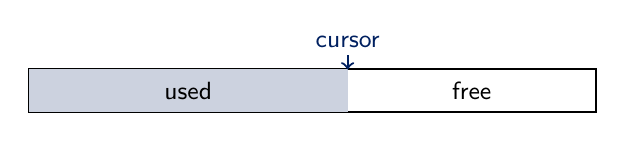
\begin{tikzpicture}[scale=0.9]
  \draw[thick] (0,0) rectangle (8,0.6);
  \fill[darkblue!20] (0,0) rectangle (4.5,0.6);
  \draw[darkblue, thick, ->] (4.5,0.8) -- (4.5,0.6) node[above, yshift=4pt]{\small cursor};
  \node at (2.25,0.3) {\small used};
  \node at (6.25,0.3) {\small free};
\end{tikzpicture}
\caption{Linear allocator state: the cursor divides the buffer into used and free regions.}
\end{figure}

\section{Pool Allocator}

\begin{definition}[Pool Allocator]
A pool allocator divides a buffer into $N$ fixed-size \emph{slots} of
size $s$. Free slots are linked in a \emph{free-list}: each free slot
stores a pointer to the next free slot. Allocation pops the head of the
list; deallocation pushes back onto the head.
\end{definition}

\textbf{Complexity}: $O(1)$ allocation, $O(1)$ deallocation.
The list is embedded in-place: no separate bookkeeping array.

The free-list is initialised in reverse order so that the first
allocation returns the slot at the lowest address:

\begin{lstlisting}[caption={Free-list initialisation (reversed)}]
for (usize i = 0; i < m_maxSlots; ++i) {
    u8* slot = m_poolStart + i * m_slotSize;
    *reinterpret_cast<u8**>(slot) = m_freeList;
    m_freeList = slot;
}
\end{lstlisting}

\textbf{Use cases}: ECS component pools, audio source instances,
particle systems --- any subsystem that creates and destroys many
identically-sized objects at high frequency.


\paragraph{Invariant 4.2 --- Slot size}

  No allocation request may exceed \texttt{m\_slotSize}.
  The pool does not track individual allocation sizes; a larger
  request would corrupt adjacent slots.



\section{Stack Allocator}

The stack allocator is structurally identical to the linear allocator
but adds the concept of a \emph{Marker}:

\begin{lstlisting}[caption={Marker-based rollback}]
Marker m = stack.setMarker();    // snapshot cursor
// ... temporaries ...
stack.freeToMarker(m);           // roll back to m
\end{lstlisting}

A marker is simply a byte offset from the buffer start (\texttt{usize}).
\texttt{freeToMarker} moves the cursor back to the saved offset,
effectively deallocating everything allocated since the marker was set.
This supports LIFO (last-in, first-out) deallocation at $O(1)$ cost.

\textbf{Use cases}: recursive descent parsing, multi-phase asset loading
where each phase's scratch memory must be freed before the next phase.

% ============================================================================
\chapter{Container Library}
% ============================================================================

\section{Dynamic Array (\texttt{Vector<T>})}

\texttt{Vector<T>} is a heap-growing array equivalent to \texttt{std::vector},
but with \texttt{IAllocator} injection. When no allocator is provided,
\texttt{operator new} / \texttt{operator delete} are used directly.

\subsubsection{Growth Strategy}

\begin{equation}
\text{newCapacity} =
\begin{cases}
  8 & \text{if current capacity} = 0 \\
  2 \times \text{current capacity} & \text{otherwise}
\end{cases}
\end{equation}

Doubling maintains amortised $O(1)$ push-back: a sequence of $n$
push-backs performs at most $2n$ element moves total.

\subsubsection{Construction and Destruction}

Elements are constructed in-place via placement-\texttt{new}:
\texttt{new (\&m\_data[m\_size]) T(value)}.
They are explicitly destroyed before deallocation:
\texttt{m\_data[i].\textasciitilde T()}.
This ensures correct behaviour for non-trivial types while remaining
compatible with the custom allocator interface.

\subsubsection{Move Semantics}

The move constructor and move assignment transfer ownership of the
underlying buffer in $O(1)$ by pointer swap, leaving the source in
a valid empty state.

\section{Hash Map (\texttt{HashMap<K,V>})}

The current \texttt{HashMap} is a \emph{linear-scan} map backed by a
\texttt{Vector<Pair>}. All operations are $O(n)$ in the number of entries.

\begin{remark}
The current implementation is intentionally simple: the expected
use-cases (editor panel registries, asset name$\to$ID tables) have at
most a few hundred entries where cache-friendly linear scan outperforms
hash table overhead. A true hash table (open addressing, Robin-Hood
probing) is planned for \texttt{v2.0} when scene complexity requires it.
\end{remark}

\section{String View (\texttt{StringView})}

\texttt{StringView} is a non-owning, read-only view into a null-terminated
string: a pointer + length pair. It performs no heap allocation. Comparison
is lexicographic and runs in $O(\min(|a|, |b|))$.

\section{Fixed String (\texttt{FixedString<N>})}

\texttt{FixedString<N>} stores at most $N-1$ characters in an inline
\texttt{char[N]} array plus a length field. There is no heap involvement.
It is used for entity names, asset paths, and any string that must be
embeddable inside a struct without pointer indirection.

% ============================================================================
\chapter{Entity-Component System (ECS)}
% ============================================================================

\section{Design Philosophy}

The ECS in Caffeine is \emph{archetype-based}: entities with the same
set of component types share a single \texttt{Archetype}. This groups
the data for all entities with a given composition contiguously in memory,
enabling iteration over a specific component type to proceed without cache
misses.

\begin{definition}[Entity]
An entity is an unsigned 32-bit integer identifier. It carries no data.
All observable state is stored in components associated with the entity.
An entity with index $\texttt{u32\_max}$ is conventionally \emph{invalid}.
\end{definition}

\begin{definition}[Component]
A component is a plain-old-data (POD) struct. It must have no virtual
methods and no hidden heap allocation. The engine enforces this by
instantiating components through typed \texttt{ComponentPool<T>} which
stores them in a \texttt{Vector<T>}.
\end{definition}

\begin{definition}[Archetype]
An archetype $\mathcal{A}$ is the set of component types associated with a
group of entities. Two entities belong to the same archetype if and only if
they possess exactly the same set of component types.
\end{definition}

\section{Component Identification}

Each component type receives a unique 32-bit ID at program initialisation
via \texttt{ComponentID::get<T>()}:

\begin{lstlisting}[caption={Type-ID registration}]
template<typename T>
static u32 get() {
    static const u32 id = nextID();  // initialised once per type
    return id;
}
\end{lstlisting}

The \texttt{static} local variable is guaranteed to be initialised exactly
once (C++11 magic statics). The counter is an \texttt{std::atomic<u32>}
to support concurrent registration from multiple translation units.
Up to 256 distinct component types are permitted.

\section{Component Set (\texttt{ComponentSet})}

A \texttt{ComponentSet} is a bitmask of component IDs. Archetype identity is
determined by comparing two \texttt{ComponentSet}s. Set operations (union,
intersection, subset test) reduce to bitwise OR, AND, and masking.

\section{Archetype Internal Structure}

Each \texttt{Archetype} contains:
\begin{itemize}
  \item A \texttt{Vector<u32>} of entity IDs (the entities belonging to it).
  \item A \texttt{PoolRegistry}: a fixed-size array of 64 pool entries,
        indexed by component ID, each entry holding a \texttt{void*} pool
        pointer and function pointers for copy, create, and remove.
\end{itemize}

\subsubsection{Removal by Swap-and-Pop}

When an entity at index $i$ is removed from an archetype, the entity at
the last position $n-1$ is moved into slot $i$. This preserves contiguity
in $O(1)$ without shifting all subsequent elements.

\begin{equation}
\text{entity}[i] \leftarrow \text{entity}[n-1]; \quad n \leftarrow n-1
\end{equation}

The same swap-and-pop is applied to every component pool for that
archetype.

\section{Command Buffer}

Structural mutations (creating or destroying entities, adding or removing
components) \emph{during iteration} would invalidate in-flight iterators.
The \texttt{CommandBuffer} defers all mutations by recording them as
\texttt{ICommand} objects:

\begin{lstlisting}[caption={Deferred entity creation}]
Entity CommandBuffer::create() {
    u32 pendingID = m_nextPendingID++;
    m_commands.pushBack(make_unique<CreateCommand>(pendingID));
    return Entity(pendingID, nullptr);  // not yet alive in world
}
\end{lstlisting}

\texttt{execute(World\&)} is called at a safe point (end of frame,
after all systems finish) to replay all recorded mutations on the live world.

\begin{specbox}{Invariant 6.1 --- Structural mutation safety}
  ECS structural mutations (entity creation/destruction, component
  add/remove) during iteration \textbf{must} go through
  \texttt{CommandBuffer}. Direct world mutation during a
  \texttt{forEach} loop is undefined behaviour.
\end{specbox}

\section{Systems}

Systems implement \texttt{ISystem} and are registered in
\texttt{SystemRegistry}. Each system exposes \texttt{onUpdate(World\&, f32 dt)}.
The world provides \texttt{forEach<C1, C2, \ldots>} which iterates over all
entities possessing the queried component types, invoking a callable
with typed references.

% ============================================================================
\chapter{Job System and Concurrency}
% ============================================================================

\section{Architecture Overview}

The job system is a \textbf{work-stealing thread pool} with three
priority levels: \texttt{Critical}, \texttt{Normal}, and \texttt{Background}.
Each worker thread has a local double-ended queue (deque) per priority level,
plus a set of global overflow queues.

\begin{figure}[H]
\centering
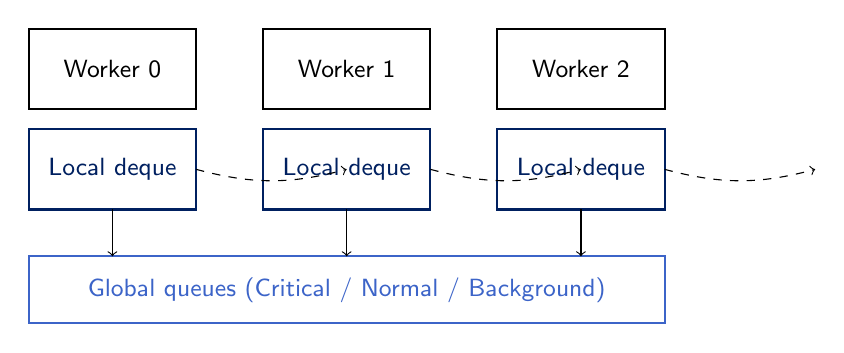
\begin{tikzpicture}[scale=0.85, every node/.style={font=\small}]
  \foreach \i in {0,1,2} {
    \draw[thick] (3.5*\i, 0) rectangle (3.5*\i+2.5, 1.2);
    \node at (3.5*\i+1.25, 0.6) {Worker \i};
    \draw[thick, darkblue] (3.5*\i, -0.3) rectangle (3.5*\i+2.5, -1.5);
    \node[darkblue] at (3.5*\i+1.25, -0.9) {Local deque};
  }
  \draw[thick, accentblue] (0, -2.2) rectangle (9.5, -3.2);
  \node[accentblue] at (4.75, -2.7) {Global queues (Critical / Normal / Background)};
  \foreach \i in {0,1,2} {
    \draw[->] (3.5*\i+1.25,-1.5) -- (3.5*\i+1.25,-2.2);
    \draw[->, dashed] (3.5*\i+2.5,-0.9) to[bend right=15] (3.5*\i+3.5+1.25,-0.9);
  }
\end{tikzpicture}
\caption{Job system topology: each worker has private local queues; dashed arrows indicate work-stealing.}
\end{figure}

\section{Work-Stealing Protocol}

On each worker tick, the following priority order is applied:

\begin{enumerate}
  \item Pop from own local queue (Critical first, then Normal, then Background).
  \item Pop from the global queue at each priority level.
  \item \textbf{Steal} from another worker's local queue (round-robin,
        from the \emph{back} of the victim's deque to minimise contention).
\end{enumerate}

Stealing from the back of the victim and consuming from the front of
self's deque is the classic Chase-Lev deque design. This minimises
contention: the owner operates on the front; stealers operate on the
back.

\section{Job Handles and the ABA Problem}

Each job is assigned a slot index and a version number.
The handle stores both. A handle is considered complete when
\texttt{m\_slots[index].flag == 1 AND m\_slots[index].version == handle.version}.
Reusing the slot for a different job increments its version, preventing
a stale handle from falsely reporting completion.


\paragraph{Invariant 7.1 --- Handle version check}

  Job handles must compare both slot index \emph{and} version number
  before reporting completion. Checking only the index is susceptible
  to ABA-style races where a recycled slot appears done prematurely.



\section{Barriers}

\texttt{JobBarrier} is a synchronisation point: a job may call
\texttt{barrier.release()} upon completion; a caller blocks on
\texttt{barrier.wait()} until the count reaches zero.
The barrier uses a \texttt{std::condition\_variable} to avoid busy-waiting.

\section{Parallel For}

\texttt{scheduleParallelFor(count, func)} divides $[0, \text{count})$
into $\min(\text{workerCount}, \text{count})$ chunks. Each chunk
$[b_i, e_i)$ is scheduled as an independent job. A shared atomic counter
tracks how many chunks have completed; the last chunk to decrement it
to zero signals the parent handle:

\begin{equation}
\text{chunkSize}_i = \left\lfloor \frac{N}{k} \right\rfloor + [i < N \bmod k]
\end{equation}

where $N$ is the total count and $k$ is the number of chunks.

\section{Worker Count}

If the caller passes 0, the system uses
$\texttt{hardware\_concurrency()} - 1$ workers, leaving one logical
core for the main thread.

% ============================================================================
\chapter{2D Physics System}
% ============================================================================

\section{Components}

\subsection{RigidBody2D}

Stores dynamic properties: \texttt{mass} $m$, \texttt{restitution} $e$,
\texttt{friction} $\mu$, \texttt{linearDamping} $d$, flags
\texttt{isKinematic} and \texttt{isSleeping}.

\subsection{Collider2D}

Stores geometric properties: \texttt{shape} (AABB or Circle),
\texttt{size}/\texttt{radius}, \texttt{offset}, collision
\texttt{layer} / \texttt{layerMask} bitmask, and flags
\texttt{isStatic}, \texttt{isTrigger}, \texttt{isOneWay}.

\section{Simulation Loop}

The system runs $k = 2$ sub-steps per frame ($k = \texttt{kSubSteps}$):

\begin{equation}
\Delta t_\text{sub} = \frac{\Delta t}{k}
\end{equation}

Per sub-step:
\begin{enumerate}
  \item Apply queued forces and impulses.
  \item Integrate velocities and positions (semi-implicit Euler).
  \item Build the spatial hash grid.
  \item Detect and resolve collisions.
  \item Update sleep state.
\end{enumerate}

\section{Integration (Semi-Implicit Euler)}

\begin{align}
  \mathbf{v}_{n+1} &= \mathbf{v}_n + \mathbf{g}\,\Delta t_\text{sub}
                    \quad (\text{gravity accumulation}) \\
  \mathbf{v}_{n+1} &\leftarrow \mathbf{v}_{n+1} \cdot \max(0,\, 1 - d\,\Delta t_\text{sub})
                    \quad (\text{linear damping}) \\
  \mathbf{x}_{n+1} &= \mathbf{x}_n + \mathbf{v}_{n+1}\,\Delta t_\text{sub}
\end{align}

The velocity is updated \emph{before} the position (semi-implicit),
which is more stable than explicit Euler for spring-like constraints.

\section{Broad-Phase: Uniform Grid}

The spatial hash maps a 2D integer cell coordinate $(c_x, c_y)$ to a
list of entity IDs. The cell coordinate of a world position $p$ is:

\begin{equation}
c = \left\lfloor \frac{p}{\texttt{kGridCellSize}} \right\rfloor
\end{equation}

with $\texttt{kGridCellSize} = 128$ world units. An entity whose AABB
spans multiple cells is inserted into all cells it touches. The cell key
is computed as:

\begin{equation}
\text{key}(c_x, c_y) = c_x \cdot 73856093 \oplus c_y \cdot 19349663
\end{equation}

(a standard spatial hashing polynomial). Candidate collision pairs are
generated by checking all pairs within the same cell, with duplicate
suppression.

\section{Narrow-Phase Geometry}

\subsection{AABB vs.\ AABB}

Let centres be $\mathbf{p}_A, \mathbf{p}_B$ with half-extents
$\mathbf{h}_A, \mathbf{h}_B$. A collision occurs when:

\begin{align}
  \text{overlapX} &= (h_{Ax} + h_{Bx}) - |p_{Bx} - p_{Ax}| > 0 \\
  \text{overlapY} &= (h_{Ay} + h_{By}) - |p_{By} - p_{Ay}| > 0
\end{align}

The separation axis is the one with \emph{minimum overlap}:

\begin{equation}
\mathbf{n} =
\begin{cases}
  (\text{sgn}(\Delta x),\, 0) & \text{if overlapX} < \text{overlapY} \\
  (0,\, \text{sgn}(\Delta y)) & \text{otherwise}
\end{cases}
\end{equation}

\subsection{Circle vs.\ Circle}

Let distance $d = |\mathbf{p}_B - \mathbf{p}_A|$ and sum of radii
$r = r_A + r_B$.

\begin{align}
  \text{collision} &\Leftrightarrow d < r \\
  \mathbf{n} &= (\mathbf{p}_B - \mathbf{p}_A) / d \\
  \text{penetration} &= r - d
\end{align}

\subsection{Circle vs.\ AABB}

The closest point on the AABB to the circle centre is:

\begin{equation}
\mathbf{c} = \text{clamp}(\mathbf{p}_\text{circle},\,
             \mathbf{p}_\text{AABB} - \mathbf{h},\,
             \mathbf{p}_\text{AABB} + \mathbf{h})
\end{equation}

If $|\mathbf{p}_\text{circle} - \mathbf{c}| < r$, a collision is detected.

\section{Impulse-Based Resolution}

Let relative velocity along the collision normal be:

\begin{equation}
v_\text{rel} = (\mathbf{v}_B - \mathbf{v}_A) \cdot \mathbf{n}
\end{equation}

If $v_\text{rel} > 0$ (separating), no impulse is applied.
Otherwise, the scalar impulse magnitude is:

\begin{equation}
j = \frac{-(1 + e)\, v_\text{rel}}{m_A^{-1} + m_B^{-1}}
\label{eq:impulse}
\end{equation}

where $e = \min(e_A, e_B)$ is the coefficient of restitution.
Velocities are updated:

\begin{align}
  \mathbf{v}_A &\leftarrow \mathbf{v}_A - j\,m_A^{-1}\,\mathbf{n} \\
  \mathbf{v}_B &\leftarrow \mathbf{v}_B + j\,m_B^{-1}\,\mathbf{n}
\end{align}

\subsubsection{Friction}

The tangential impulse $j_t$ is:

\begin{equation}
j_t = \frac{-v_\text{rel,tan}}{m_A^{-1} + m_B^{-1}},
\quad \mu = \sqrt{\mu_A \mu_B}
\end{equation}

Applied as a Coulomb friction cone: $|j_t| \leq \mu |j|$.

\section{Positional Correction (Baumgarte)}

To prevent sinking, the positions are corrected proportionally to the
penetration depth, with a slop tolerance $\delta_\text{slop}$ and
factor $k_\text{B}$:

\begin{equation}
\Delta\mathbf{x} = \frac{(\text{penetration} - \delta_\text{slop}) \cdot k_\text{B}}{m_A^{-1} + m_B^{-1}}\,\mathbf{n}
\end{equation}

with $\delta_\text{slop} = 0.01$ and $k_\text{B} = 0.4$.

\section{Sleep System}

An entity enters sleep when its velocity magnitude drops below
$v_\text{sleep} = 0.05$ for longer than $t_\text{sleep} = 0.5\,\text{s}$.
A sleeping entity skips integration entirely, saving compute for
static scenes with many resting bodies. Any external force or impulse
wakes the entity immediately.

\section{Raycast}

A ray $\mathbf{r}(t) = \mathbf{o} + t\hat{\mathbf{d}}$ is tested against
all entities with a \texttt{Collider2D}. For AABB colliders the
slab method is used; for circle colliders the quadratic form:

\begin{equation}
|(\mathbf{o} + t\hat{\mathbf{d}}) - \mathbf{c}|^2 = r^2
\end{equation}

is solved for $t$. The hit with minimum $t \geq 0$ is returned.

% ============================================================================
\chapter{Spatial Audio System}
% ============================================================================

\section{Architecture}

The audio system wraps SDL3's \texttt{SDL\_AudioStream} API. It maintains
a pool of \texttt{AudioSource} objects (default 32 SFX channels).
Each source maps to one \texttt{SDL\_AudioStream} bound to the system's
\texttt{SDL\_AudioDeviceID} (default device, S16 stereo 44100\,Hz).

\section{AudioClip}

An \texttt{AudioClip} is a pure descriptor: a pointer to raw PCM bytes,
size, sample rate, channel count, bits per sample, and duration.
The system does not own the memory; clips are registered by the asset
pipeline which manages their lifetimes.

\section{Spatial Attenuation}

For an emitter at world position $\mathbf{p}_e$ and listener at
$\mathbf{p}_l$ with maximum audible distance $d_\text{max}$:

\begin{equation}
\text{volume} = \max\!\left(0,\; 1 - \frac{|\mathbf{p}_e - \mathbf{p}_l|}{d_\text{max}}\right)
\label{eq:audio-volume}
\end{equation}

This is a \emph{linear falloff} model. Physically accurate inverse-square
falloff ($1/d^2$) sounds too aggressive for game contexts; linear falloff
produces a smoother perceptual transition.

\section{Stereo Panning}

The pan value in $[-1, 1]$ is derived from the horizontal offset of the
emitter relative to the listener:

\begin{equation}
\text{pan} = \text{clamp}\!\left(\frac{p_{ex} - p_{lx}}{d_\text{max}},\; -1,\; 1\right)
\end{equation}

Gain for each channel:
\begin{align}
  g_L &= v \cdot (1 - \max(0, \text{pan})) \\
  g_R &= v \cdot (1 + \min(0, \text{pan}))
\end{align}

The stream gain is set to $\max(g_L, g_R)$. True per-channel gain
requires a custom mixing callback (planned).

\section{Playback Loop}

When a looping source exhausts its buffer (SDL reports
\texttt{SDL\_GetAudioStreamAvailable} == 0), the full clip data is
re-submitted via \texttt{SDL\_PutAudioStreamData}. The implementation
tracks elapsed time to detect this condition frame-accurately.

% ============================================================================
\chapter{Asset Pipeline (.caf Format)}
% ============================================================================

\section{Design Goals}

The Caffeine Asset Format (\texttt{.caf}) is a \textbf{zero-parsing,
zero-copy} binary container. The layout on disk is a direct mirror of
the in-RAM / in-VRAM layout, so loading is a single \texttt{fread} followed
by pointer arithmetic --- no deserialization step, no allocations beyond
the buffer itself.

\section{File Layout}

\begin{equation*}
\underbrace{[0\ldots 31]}_{\text{CafHeader}}
\underbrace{[32\ldots 32+N-1]}_{\text{Metadata}}
\underbrace{[32+N\ldots 32+N+M-1]}_{\text{Payload}}
\underbrace{[32+N+M\ldots 32+N+M+3]}_{\text{Footer CRC32}}
\end{equation*}

\begin{table}[H]
\centering
\caption{CafHeader fields (32 bytes, little-endian)}
\begin{tabular}{lllr}
\toprule
\textbf{Offset} & \textbf{Field} & \textbf{Type} & \textbf{Bytes} \\
\midrule
0  & \texttt{magic}        & \texttt{u32} (= 0xCAFECAFE) & 4 \\
4  & \texttt{versionMajor} & \texttt{u16}                & 2 \\
6  & \texttt{versionMinor} & \texttt{u16}                & 2 \\
8  & \texttt{type}         & \texttt{AssetType} (u16)    & 2 \\
10 & \texttt{flags}        & \texttt{CafFlags} (u16)     & 2 \\
12 & \texttt{crc32}        & \texttt{u32}                & 4 \\
16 & \texttt{metadataSize} & \texttt{u64}                & 8 \\
24 & \texttt{dataSize}     & \texttt{u64}                & 8 \\
\bottomrule
\end{tabular}
\end{table}

\begin{specbox}{Invariant 10.1 --- Endianness}
  The \texttt{.caf} format is little-endian.
  A \texttt{static\_assert} verifies \texttt{std::endian::native == std::endian::little}
  at compile time; the format must not be used on big-endian platforms
  without byte-swapping shims.
\end{specbox}

\section{Integrity Verification}

Two CRC32 checks are performed at load time:
\begin{enumerate}
  \item \textbf{Payload CRC32}: \texttt{crc32(payload, dataSize)} must equal
        \texttt{header.crc32}.
  \item \textbf{Whole-file CRC32}: The 4-byte footer stores
        \texttt{crc32(everything-before-footer)}, providing end-to-end
        integrity against file corruption or truncation.
\end{enumerate}

The CRC32 uses the IEEE 802.3 polynomial $P = \texttt{0xEDB88320}$
(reflected form). The lookup table of 256 entries is built at
compile time via a \texttt{constexpr} function, adding zero run-time
initialisation cost.

\begin{specbox}{Invariant 10.2 --- CRC32 verification}
  Both CRC32 checks must pass before any \texttt{.caf} file is used.
  A file that passes only one check is treated as corrupt.
\end{specbox}

\section{Asset Types}

\begin{table}[H]
\centering
\caption{AssetType discriminants and their metadata structs}
\begin{tabular}{lll}
\toprule
\textbf{Type} & \textbf{Metadata struct} & \textbf{Notes} \\
\midrule
\texttt{Texture}   & \texttt{TextureMetadata} (24 B)  & width, height, format, mips \\
\texttt{Audio}     & \texttt{AudioMetadata} (16 B)    & sampleRate, channels, samples \\
\texttt{Mesh}      & (Phase 5)                        & vertex / index buffers \\
\texttt{Prefab}    & \texttt{SceneMetadata} (20 B)    & binary ECS entity template \\
\texttt{Scene}     & \texttt{SceneMetadata} (20 B)    & full world state snapshot \\
\texttt{Shader}    & \texttt{ShaderMetadata} (8 B)    & stage (vert/frag/compute) \\
\texttt{Animation} & (planned)                        & animation clip frames \\
\bottomrule
\end{tabular}
\end{table}

\section{Live Asset Watching}

\texttt{FileWatcher} monitors a directory via
\texttt{ReadDirectoryChangesW} (Windows) or a polling stub (other
platforms). Changed paths are pushed onto a thread-safe queue and polled
from the main thread so that the asset loader can hot-reload without
cross-thread world mutation.

% ============================================================================
\chapter{Game Loop}
% ============================================================================

\section{Fixed Timestep with Interpolation}

The game loop implements a \textbf{fixed-timestep with remainder
interpolation} --- the pattern described by Glenn Fiedler in
``Fix Your Timestep'' (2004).

\begin{lstlisting}[caption={Game loop tick}]
accumulator += min(deltaTime, maxFrameTime);
while (accumulator >= fixedDeltaTime) {
    fixedUpdate(fixedDeltaTime);
    accumulator -= fixedDeltaTime;
}
alpha = accumulator / fixedDeltaTime;
render(alpha);
\end{lstlisting}

\subsubsection{Spiral of Death Protection}

Clamping $\Delta t$ to \texttt{maxFrameTime} (default $0.25\,\text{s}$)
prevents the \emph{spiral of death}: if a frame takes longer than
$\Delta t_\text{fixed}$, the accumulator would grow without bound,
scheduling infinitely many fixed-update steps, making the frame even
longer. The clamp trades simulation accuracy (the simulation slows
down in real time) for stability.

\subsubsection{Interpolation Alpha}

$\alpha = \texttt{accumulator} / \Delta t_\text{fixed} \in [0, 1)$
is the fraction of a fixed step that has elapsed but not yet been
simulated. The renderer uses it to interpolate between the previous
and current physics state for sub-frame smooth visual output.

\section{Debug Hook Registry}

\texttt{DebugHookRegistry} provides a single-slot registration for an
\texttt{IDebugHooks} implementation. The core engine calls hooks
unconditionally-if-registered:

\begin{lstlisting}[caption={Zero-overhead hook call pattern}]
if (auto* h = DebugHookRegistry::hooks()) {
    h->onFrameEnd(stats);
}
\end{lstlisting}

This decouples the core from the editor without requiring a virtual
call on every path: when no hooks are registered (shipped game), the
branch is predicted-not-taken with negligible cost.

% ============================================================================
\chapter{Editor and Scene Viewport}
% ============================================================================

\section{Overview}

The scene viewport (\texttt{SceneViewport}) is a 100\% software-rendered
panel driven by ImGui's \texttt{ImDrawList}. There is no GPU projection
matrix; all world-to-screen transformations are implemented analytically
in the \texttt{projectToScreen} function. Three view modes are supported:
\textbf{Mode2D} (orthographic top-down), \textbf{Mode3D} (perspective
orbit), and \textbf{Isometric} (dimetric projection).

\section{Camera Model}

The camera state is stored in \texttt{EditorContext}:

\begin{table}[H]
\centering
\caption{Camera state variables}
\begin{tabular}{lll}
\toprule
\textbf{Variable} & \textbf{Type} & \textbf{Meaning} \\
\midrule
\texttt{camYaw}      & \texttt{f32} & Azimuth angle (radians, Y-axis) \\
\texttt{camPitch}    & \texttt{f32} & Elevation angle (radians, X-axis), clamped to $[-\pi/2, \pi/2]$ \\
\texttt{camFocus}    & \texttt{Vec3} & World-space point the camera orbits \\
\texttt{camDistance} & \texttt{f32} & Distance from focus to eye \\
\bottomrule
\end{tabular}
\end{table}

\section{projectToScreen --- Mode2D}

In 2D mode, the projection is a simple affine pan-and-zoom:

\begin{align}
  s_x &= \text{origin}_x + \frac{W}{2} + p_x \cdot \text{zoom} + \text{panX} \\
  s_y &= \text{origin}_y + \frac{H}{2} - p_y \cdot \text{zoom} + \text{panY}
\end{align}

where $W, H$ are the viewport dimensions and $(p_x, p_y)$ is the world
position.

\section{projectToScreen --- Mode3D}

The 3D projection is a software perspective transform using the
camera's spherical parameterisation.

\subsubsection{Step 1: Translate to Camera-Relative Space}

\begin{equation}
\mathbf{r} = \mathbf{p} - \mathbf{f}
\end{equation}

where $\mathbf{f} = \texttt{camFocus}$.

\subsubsection{Step 2: Yaw Rotation (Y-axis, angle $\psi$)}

\begin{align}
v_x &=  \cos\psi \cdot r_x + \sin\psi \cdot r_z \\
v_y &= r_y \\
v_z &= -\sin\psi \cdot r_x + \cos\psi \cdot r_z
\end{align}

The yaw rotation brings the camera's viewing direction along the $+Z$ axis
in view space.

\subsubsection{Step 3: Pitch Rotation (X-axis, angle $\phi$)}

\begin{align}
v_{y2} &=  \cos\phi \cdot v_y + \sin\phi \cdot v_z \\
v_{z2} &= -\sin\phi \cdot v_y + \cos\phi \cdot v_z
\end{align}

\subsubsection{Step 4: Perspective Divide}

The viewing volume is parameterised by \texttt{camDistance} $D$:

\begin{equation}
\text{fovScale} = \frac{s \cdot D}{\max(D + v_{z2},\; \varepsilon)}
\label{eq:fovscale}
\end{equation}

where $s = \min(W, H) / 2$ is the half-screen size used as a scale
factor, and $\varepsilon = 0.01$ guards against division by zero.
The screen coordinates are:

\begin{align}
  s_x &= c_x + v_x \cdot \text{fovScale} + \text{panX} \\
  s_y &= c_y - v_{y2} \cdot \text{fovScale} + \text{panY}
\end{align}

\subsubsection{Near-Plane Clipping}

A point is \emph{behind the camera} when $D + v_{z2} \leq \varepsilon$.
For line segments (grid, gizmo axes), this causes \texttt{fovScale} to
approach infinity, projecting to extreme screen positions.
The fix is near-plane clipping: for a segment $(\mathbf{a}, \mathbf{b})$,
compute the camera-depth of each endpoint $d_A, d_B$. If exactly one
endpoint is behind the near plane (depth $< \varepsilon$), linearly
interpolate the segment to the boundary:

\begin{equation}
t = \frac{\varepsilon - d_A}{d_B - d_A}, \quad
\mathbf{c} = \mathbf{a} + t(\mathbf{b} - \mathbf{a})
\end{equation}

The clipped segment $(\mathbf{c}, \mathbf{b})$ (or $(\mathbf{a}, \mathbf{c})$)
is then safe to project without numerical explosion.

\begin{specbox}{Invariant 12.1 --- Near-plane clipping}
  Near-plane clipping must be applied to every projected line segment
  in Mode3D. Skipping it for ``short'' segments is not safe; the
  perspective divide can still explode for world-space points near
  the camera position.
\end{specbox}

\section{projectToScreen --- Isometric}

The isometric projection uses a fixed dimetric angle offset of
$\alpha_0 = 30^\circ = \pi/6$ added to the azimuth:

\begin{align}
  \cos A &= \cos(\psi + \alpha_0) \quad\text{(effective azimuth)} \\
  \sin A &= \sin(\psi + \alpha_0) \\
  s_x &= c_x + (r_x \cdot \cos A + r_z \cdot \sin A) \cdot \text{zoom} + \text{panX} \\
  s_y &= c_y - (r_y - r_x \cdot \sin A \cdot 0.5 + r_z \cdot \cos A \cdot 0.5) \cdot \text{zoom} + \text{panY}
\end{align}

This produces the classic isometric look without using a GPU depth buffer.

\section{Infinite Grid Rendering}

The 3D grid is drawn on the XZ plane ($y = 0$). Grid lines are world
segments of the form:

\begin{align}
  &\{(i, 0, z) : z \in [-H, H]\} \quad \text{(X-aligned lines)} \\
  &\{(x, 0, i) : x \in [-H, H]\} \quad \text{(Z-aligned lines)}
\end{align}

where $i \in \{-H_\text{lines}, \ldots, H_\text{lines}\}$ and
$H_\text{lines}$ is chosen dynamically based on \texttt{camDistance}.

Each segment is near-plane clipped before projection. The adaptive
spacing doubles when the grid density exceeds 60 lines on screen:

\begin{equation}
\text{spacing} \leftarrow 2 \cdot \text{spacing}
\quad \text{while } \frac{2 \cdot H_\text{lines}}{\text{spacing}} > 60
\end{equation}

\section{Transform Gizmo}

The \texttt{TransformGizmo} renders translate, rotate, and scale handles
directly on the \texttt{ImDrawList}. For each axis $A \in \{X, Y, Z\}$,
the tip position is computed by projecting the world point
$\mathbf{p} + \Delta A \cdot \hat{\mathbf{e}}_A$ through
\texttt{projectToScreen}.

\subsubsection{Axis Normalisation}

To keep handles at a constant screen-space length $L$ (pixel units),
the raw projected tip is normalised:

\begin{equation}
\text{end}_A = \mathbf{o} + L \cdot \frac{\text{rawEnd}_A - \mathbf{o}}{|\text{rawEnd}_A - \mathbf{o}|}
\end{equation}

If $|\text{rawEnd}_A - \mathbf{o}| < 3\,\text{px}$ (the axis projects
nearly onto the screen-space origin), a per-axis fallback direction is used.

\subsubsection{Z-Axis Overlap Guard}

When the Z-axis fallback direction projects to within
$0.3 \cdot L$ pixels of the Y-axis endpoint, the Z-axis is forced to
its default fallback ($-0.6L, +0.6L$) to avoid ambiguity:

\begin{equation}
d_{ZY} = |\text{end}_Z - \text{end}_Y| < 0.3L
\implies \text{end}_Z \leftarrow \text{fallback}_Z
\end{equation}

\section{Navigation Widget (Orientation Gizmo)}

The mini orientation gizmo in the viewport corner shows the camera's
current viewing direction. Each world axis is projected onto screen space
using the camera rotation only (no perspective divide):

\begin{align}
  s_x    &=  \cos\psi \cdot A_x + \sin\psi \cdot A_z \\
  s_{y1} &= A_y \\
  s_z    &= -\sin\psi \cdot A_x + \cos\psi \cdot A_z \\
  s_{y2} &= \cos\phi \cdot s_{y1} + \sin\phi \cdot s_z \\
  \text{dir} &= \left(\frac{s_x}{L},\; \frac{-s_{y2}}{L}\right) \cdot L_\text{widget}
\end{align}

where $(A_x, A_y, A_z)$ is the world-space direction of the axis (e.g.\
$(1, 0, 0)$ for X), $\psi$ and $\phi$ are \texttt{camYaw} and
\texttt{camPitch}, and $L_\text{widget} = 22\,\text{px}$ is the display
length.

The three axes are drawn in fixed colours: X red (255, 70, 70),
Y green (70, 255, 90), Z blue (90, 140, 255).

\begin{specbox}{Invariant 12.2 --- Navigation widget correctness}
  Navigation widget axis directions must be computed from the live
  \texttt{camYaw} and \texttt{camPitch} values every frame.
  Hardcoding or caching the directions between frames is incorrect.
\end{specbox}

\section{Keyboard Navigation}

Arrow key navigation moves \texttt{camFocus} in the camera's horizontal
plane (pitch is ignored for navigation to avoid tilting the focus point
out of the ground plane):

\begin{align}
  \Delta\mathbf{f}_\text{forward}  &= (-\sin\psi,\; 0,\;  \cos\psi) \cdot v \\
  \Delta\mathbf{f}_\text{right}    &= ( \cos\psi,\; 0,\;  \sin\psi) \cdot v
\end{align}

The \texttt{ImGuiWindowFlags\_NoNavInputs} flag on the viewport window
prevents ImGui from consuming arrow key events to navigate UI buttons.

% ============================================================================
\chapter{Editor Architecture and Undo System}
% ============================================================================

\section{EditorContext}

\texttt{EditorContext} is the singleton shared state passed to every
panel. It holds selection state, gizmo mode, snap settings, the camera
parameters described in Chapter~12, and the
\texttt{UndoStack}.

\section{UndoStack}

The undo system uses \textbf{full world snapshots}: each
\texttt{EditorCommand} stores a \texttt{beforeState} and \texttt{afterState}
as \texttt{std::vector<u8>} binary blobs. Undo restores the before state;
redo restores the after state.

The ring buffer holds up to 256 commands. A new push after an undo
truncates the redo history (linear undo). This is the simplest correct
implementation; a command-specific delta approach (e.g.\ storing only
the modified component fields) would be more memory-efficient but
requires serialisation round-trips for every component type.

\section{Panel System}

Each editor panel is an autonomous class with an
\texttt{onImGuiRender(World\&, EditorContext\&)} method:
\texttt{HierarchyPanel}, \texttt{InspectorPanel}, \texttt{AssetBrowser},
\texttt{AnimationTimeline}, \texttt{AudioPreviewPanel},
\texttt{BuildDialog}, etc.
Panels communicate solely through \texttt{EditorContext}; no panel holds
a pointer to another panel.

% ============================================================================
\chapter{Implementation Rules and Future Specifications}
% ============================================================================

\section{Binding Invariants}

The following invariants must be preserved by all future implementations.
A proposed change that violates any invariant requires explicit discussion
and this document must be updated before implementation begins.

\begin{table}[H]
\centering
\caption{Binding invariants summary}
\begin{tabular}{lp{9cm}}
\toprule
\textbf{ID} & \textbf{Statement} \\
\midrule
I-1  & All type widths validated by \texttt{static\_assert}. \\
I-2  & \texttt{CF\_ASSERT} is never removed to silence errors. \\
I-3  & Allocator alignment is always a power of two $\geq 8$. \\
I-4  & Pool slot size is never exceeded at the call site. \\
I-5  & Component IDs are registered atomically; no component may receive two different IDs. \\
I-6  & ECS structural mutations during iteration go through \texttt{CommandBuffer}. \\
I-7  & Job handles must check version equality before reporting completion. \\
I-8  & \texttt{.caf} files are always verified with both CRC32 checks before use. \\
I-9  & Near-plane clipping is applied to every projected line segment in Mode3D. \\
I-10 & Navigation widget axes are computed from live \texttt{camYaw}/\texttt{camPitch} values, never hardcoded. \\
\bottomrule
\end{tabular}
\end{table}

\section{Planned Systems}

The following systems are specified here to constrain future
implementation choices, even though they are not yet implemented.

\subsection{Mesh Rendering (Phase 5)}

Mesh assets store interleaved vertex data (position, normal, UV, tangent)
aligned to 32 bytes for AVX2 SIMD. The RHI layer (\texttt{src/rhi/})
wraps SDL3-GPU command buffers; mesh rendering will use indexed draws
with a single persistent vertex buffer per mesh, uploaded once at asset
load time.

\subsection{Scripting (Lua 5.4)}

The scripting engine (\texttt{src/script/}) embeds Lua 5.4.
Each entity may have a \texttt{ScriptComponent} that stores a Lua table
as its instance state. The engine exposes the ECS world to scripts via a
C API binding layer. Script execution runs on the main thread; no
cross-thread Lua state sharing is permitted.

\subsection{Animation}

Animation clips store keyframe data (time, value, tangent for Hermite
interpolation) per channel (position, rotation, scale). The
\texttt{AnimationSystem} evaluates clips via the Hermite spline formula
and writes results into transform components.

% ============================================================================
\chapter*{Bibliography}
\addcontentsline{toc}{chapter}{Bibliography}
% ============================================================================

\begin{enumerate}[label={[\arabic*]}]
  \item G.\ Fiedler, ``Fix Your Timestep!'', \emph{Gaffer on Games}, 2004.
        \url{https://gafferongames.com/post/fix_your_timestep/}

  \item K.\ Shoemake, ``Animating Rotation with Quaternion Curves,''
        \emph{SIGGRAPH 1985 Proceedings}, ACM, pp.\ 245--254, 1985.

  \item D.\ Eberly, \emph{3D Game Engine Architecture}, Morgan Kaufmann, 2005.

  \item B.\ Mirtich, ``Impulse-Based Dynamic Simulation of Rigid Body Systems,''
        Ph.D.\ thesis, University of California, Berkeley, 1996.

  \item M.\ Dickheiser (ed.), \emph{Game Programming Gems 6},
        Charles River Media, 2006.
        (Chapter on work-stealing schedulers.)

  \item SDL3 Documentation, \url{https://wiki.libsdl.org/SDL3/FrontPage}

  \item Dear ImGui, \url{https://github.com/ocornut/imgui}

  \item ISO/IEC 14882:2020, \emph{Programming Languages --- C++}, 2020.
\end{enumerate}


\end{document}
